\chapter{HIP Runtime API} \label{chap:HIP_runtime_API}

在本書的前三章中,我們了解到 HIP 程式由在 CPU 上運行的host部分和在 GPU 上執行的device部分組成。上一章探討了如何設計 GPU kernel程式的方法。本章將介紹如何利用 HIP Runtime API 來增強host程式對 GPU 的控制能力。

\section{HIP的記憶體管理}
在目前為止的範例中,我們採用了 HIP 提供的預設記憶體配置方式。然而,HIP 提供了更靈活的記憶體配置選項。當處理 GPU 時,這種靈活性尤其重要,因為高效的記憶體傳輸與存取對性能至關重要。

\subsection{Pinned Memory}
在本節中,我們將探索pinned memory的概念及其在優化 CPU 和 GPU 之間資料傳輸性能中的重要性。透過了解和使用pinned memory,我們可以克服一些與分頁記憶體(pageable memory)相關的性能開銷。

當記憶體使用 malloc 函數配置時,通常會位於分頁記憶體中,這些記憶體會在需要釋放物理記憶體時被系統交換到磁碟。然而,這種行為可能會導致顯著的性能開銷,特別是在頻繁進行 CPU 和 GPU 之間資料傳輸的程式中。為了解決這個問題,我們可以利用pinned memory。HIP API 提供了一個 \term{hipHostMalloc} 函數,讓我們能夠在host上分配pinned memory。該函數有三個參數:一個指向已分配記憶體的指標、要分配的記憶體大小以及一個選擇性的標誌用以指定分配類型,如 Listing 4.1 所示。pinned memory是在物理記憶體被存放在固定位置的記憶體。與傳統的分頁記憶體不同,pinned memory始終保持在其被指定的物理位置,因此不需要頻繁移動資料。host和device都可以訪問已分配的記憶體。

\begin{lstlisting}[language=C, caption={在HIP中使用pinned memory進行記憶體配置}, label={1st:example}]
float *a;
hipHostMalloc(&a, bytes, usinged int flags);
\end{lstlisting}

使用pinned memory在host與device之間需要頻繁資料傳輸的情況下別具優勢。pinned memory可以透過加快記憶體訪問速度顯著提升資料傳輸性能,進而增強程式的整體效能。\term{hipMemcpy()} 和 \term{hipMemcpyAsync()} 搭配pinned memory,可以為host與device之間的資料傳輸提供一種高效的機制。需要注意的是,使用 \term{hipHostMalloc()} 分配的pinned memory應使用 \term{hipHostFree()} 函數來釋放記憶體,而非標準的 free 函數。這樣可以確保正確釋放pinned memory,並將其從指定的物理位置中鬆綁。如果嘗試用 \term{free()} 函數釋放pinned memory,可能會導致問題,因為 \term{free()} 無法解除記憶體的固定狀態。

\begin{lstlisting}[language=C, caption={釋放pinned memory}, label={2nd:example}]
hipHostFree(d_a);
\end{lstlisting}


為了展示pinned memory的實際應用,讓我們審視一個使用這種記憶體類型的向量加法示例。截至目前,本節已討論了使用pinned memory的優勢,並指出其如何提升 GPU 性能。為了在向量加法中有效利用pinned memory,我們需要修改記憶體分配過程。不像Listing 2.5使用傳統的 \term{malloc()} 函數,而是採用 Listing 4.3 提供的程式碼片段。這段更新的程式碼確保記憶體分配是透過pinned memory完成的,從而為向量加法程式帶來效益。

\begin{lstlisting}[language=C, caption={在向量加法範例中使用host記憶體配置}, label={3rd:example}]
// 在host上為每個向量分配記憶體
HIP_ASSERT(hipHostMalloc(&CPUArrayA, bytes));
HIP_ASSERT(hipHostMalloc(&CPUArrayB, bytes));
HIP_ASSERT(hipHostMalloc(&CPUArrayC, bytes));
HIP_ASSERT(hipHostMalloc(&CPUVerifyArrayC, bytes));
\end{lstlisting}

透過使用 hipHostMalloc() 函數,我們可以使用pinned memory來分配host記憶體。這確保記憶體被分配在實體記憶體中,並消除了 CPU 和 GPU 之間頻繁的資料傳輸需求,從而提升性能。此外,我們必須在記憶體釋放部分進行更改。與 Listing 2.6 所示的傳統 host記憶體釋放方法不同,我們將使用 hipHostFree() 函數,如 Listing 4.4 所述。然而, device記憶體的釋放方法將保持不變。

\begin{lstlisting}[language=C, caption={釋放hostpinned memory}, label={4th:example}]
// 釋放host記憶體
hipHostFree(CPUArrayA);
hipHostFree(CPUArrayB);
hipHostFree(CPUArrayC);
\end{lstlisting}

透過利用pinned memory,我們可以優化向量加法程式範例中的記憶體分配過程。這使我們能夠充分利用pinned memory提供的優勢,例如提高資料傳輸性能和減少開銷。此外,使用 hipHostFree 函數正確釋放記憶體可確保高效的記憶體管理。

\subsection{Unified Memory}

為了進一步促進host與device之間的通信,HIP 提供了unified memory。這種抽象化簡化了host與device記憶體之間的資料複製過程。手動在host與device記憶體之間的資料搬移既耗時又容易出錯,並且需要額外的程式設計工作量。而unified memory為此挑戰提供了一種高效的解決方案。

HIP 的unified memory提供了一個CPU和GPU都能訪問的統一地址空間。透過unified memory,資料可以被host與device無縫地訪問,而不需要顯式的資料複製。這消除了手動記憶體複製的負擔,並簡化了資料管理。要分配unified memory,我們可以使用 \term{hipMallocManaged()} 函數,如 Listing 4.5 所示。該函數接受一個指向分配記憶體位置的指標以及分配記憶體的大小。使用受管理的記憶體時,CPU與GPU之間的資料遷移是被透明處理的。當 GPU 訪問記憶體時,資料會自動被搬移到device;而當 CPU 訪問記憶體時,資料會搬移回host。這種動態搬移確保了資料的可用性並優化了記憶體利用率。使用unified memory使開發者能夠編寫無需顯式記憶體管理、並無縫發揮 GPU 強大計算能力的程式。這大大降低了程式的複雜性,並簡化了開發過程。

\begin{lstlisting}[language=C, caption={在HIP中使用unified memory進行記憶體配置}, label={5th:example}]
int *a;
hipMallocManaged(&a, bytes);
\end{lstlisting}

為了更好地理解unified memory的使用,我們將探討一個基於之前的向量加法情境,並使用unified memory的範例。在這個範例中,我們將利用unified memory創建一個可被 CPU 和 GPU 同時訪問的單一記憶體空間。為此,我們將使用 \term{hipMallocManaged} 函數。在先前 Listing 2.5 中的向量加法範例中,記憶體分配是分別在 CPU 和 GPU 進行的,分別使用 malloc 和 hipMalloc 函數。然而,我們可以透過使用 hipMallocManaged 函數來簡化這個過程,因該函數分配的記憶體可以同時被 CPU 和 GPU 訪問。我們可以用如 Listing 4.6 所示的程式碼片段替換 CPU 和 GPU 的記憶體分配程式碼。由於 CPU 和 GPU 都可以訪問unified memory,因此不需要進行記憶體複製。

\begin{lstlisting}[language=C, caption={在HIP中使用unified memory進行記憶體配置}, label={6th:example}]
// 每個vector的大小 (byte)
size_t bytes = n * sizeof(double);

// 為每個向量分配unified memory
float *a, *b, *c, *cpuVerifyC;
hipMallocManaged(&a, bytes);
hipMallocManaged(&b, bytes);
hipMallocManaged(&c, bytes);
hipMallocManaged(&cpuVerifyC, bytes);

// 初始化向量
for(int i = 0; i < n; i++) {
    a[i] = i;
    b[i] = i;
}
\end{lstlisting}

與我們之前的範例類似,在釋放記憶體時,不再需要分別釋放host端和device端的記憶體。只需使用 hipFree() 函數釋放記憶體即可。

\begin{lstlisting}[language=C, caption={釋放unified memory}, label={7th:example}]
// 釋放記憶體
hipFree(a);
hipFree(b);
hipFree(c);
hipFree(cpuVerifyC);
\end{lstlisting}

透過使用 hipMallocManaged 的unified memory,我們可以簡化記憶體分配流程,創建一個可供 CPU 和 GPU 共用的unified memory空間。這消除了 CPU 和 GPU 各自獨立分配記憶體以及在它們之間顯式複製記憶體的需求,從而使程式碼更簡潔。此外,透過使用 hipFree() 函數,我們可以高效地釋放unified memory。我們討論了如何將這種方法應用於向量加法範例,從而簡化記憶體管理並提升 GPU 程式設計的整體效率。

\section{HIP streams}

現代 GPU 為程式設計者提供了並行 kernel 以及重疊計算與通信的靈活性。這種能力可帶來顯著的性能提升。許多實際應用使用 kernel 處理獨立的資料結構,一個 kernel 的輸入不一定依賴於另一個 kernel 的輸出。因此,程式設計者可以選擇並行多個 kernel 以最大化 GPU 的利用率。此外,在早先完成處理的 kernel 將資料傳回host的同時,還可以啟動第二個 kernel。此功能利用了 HIP streams。在本節中,我們將了解它們的工作原理以及 GPU 程式設計者可以如何利用它們來提升應用程式性能。

\subsection{stream 的基本}
HIP 的操作,如資料傳輸和 kernel 啟動,依賴於 HIP Streams。一個stream中的所有操作都按照應用程式指定的順序執行。截至目前,我們一直使用預設的stream,也稱為 NULL stream或stream 0。我們可以回顧第二章的討論,我們將 kernel 啟動參數列表中的stream參數設置為 0。HIP 程式設計模型指出在預設情況下,所有操作都在 NULL stream中執行。然而,程式設計者可以為資料傳輸和記憶體複製指定stream。

HIP stream提供以下功能:
\begin{itemize}
    \item stream可以重疊資料溝通和 kernel 啟動。舉例來說,程式設計者可以在stream 1 中啟動一個 kernel,並在stream 2 中複製某個在stream 2 啟動的 kernel 的資料。如果只使用預設的 NULL stream,程式設計者必須等到記憶體複製完成後才能啟動下一個 kernel。
    \item stream可以同時分派多個 kernel以最大化 GPU 的利用率。此功能對於包含無法完全利用 GPU 資源的小型 kernel 的應用程式尤其重要。
\end{itemize}

值得注意的是,從程式設計者的角度來看,所有程式流是同時執行的。然而,實際執行順序取決於排程(由 GPU 驅動程式和 GPU 硬體進行),以及硬體資源的可用性(例如,記憶體複製引擎的數量)。

在深入討論 HIP stream 之前,請記住以下兩個要點:
\begin{itemize}
    \item Kernel 啟動是非同步的。因此,在 kernel 執行後,程式控制會立即返回host端。這就是為什麼我們在 kernel 啟動後使用 \term{hipDeviceSynchronize} 來同步host和device的原因。這同時確保 kernel 在執行後續程式碼之前完成執行。
    \item 到目前為止,\bold{hipMemcpy} 命令是同步的。因此,host會阻塞執行直到記憶體傳輸完成。然而,HIP 提供了支援host與device之間非同步傳輸的 API,但需使用多個streams。我們將在接下來的章節中探討這一功能,因為它可以提高並行性並改進應用程式效能。
\end{itemize}

\subsection{關鍵的stream 相關 API}
現在我們來探討一些最常見的HIP API,並討論如何有效地使用它們

\bold{創建與關閉stream}
程式設計者需要負責建立streams並在使用完成後關閉它們。stream的建立是透過 \term{hipStreamCreate} API,其參數為 \term{hipStream\_t} 型別的變數,如 Listing 4.8 所示。同樣地,stream的終止使用 \term{hipStreamDestroy} API,其參數也為 \term{hipStream\_t} 型別的變數。在所有對stream的操作完成後,呼叫 \term{hipStreamDestroy} 是一種良好的程式設計習慣。

\begin{lstlisting}[language=C, caption={創建與關閉stream}, label={8th:example}]
hipStream_t myStream;
hipStreamCreate(&myStream);

// 使用stream

hipStreamDestroy(&myStream);
\end{lstlisting}

在使用多個streams 時,開發者可能希望暫停host端的處理,直到特定stream中的 kernel 完成執行。對於host CPU 而言,這種序列化是必要的,特別是在 CPU 需要該stream的輸出以進行host端處理時。為了支援這種序列化,HIP 提供了 \term{hipStreamSynchronize} API,該 API 接受我們希望同步的stream物件作為參數。如果開發者不想阻塞host CPU,但希望同步多個streams,可以使用 \term{hipStreamWaitEvent} API(將在 4.3 節中介紹)。

\bold{非同步的記憶體複製}
要充分發揮streams的潛力需要了解非同步記憶體複製的工作原理。截至目前,我們已使用 \term{hipMemcpy} API 在 host CPU 和 GPU 之間傳輸資料。這是一種阻塞式呼叫,程式控制在資料傳輸完成之前不會返回 host。相反地,\term{hipMemcpyAsync} 是非阻塞的。該 API 執行的任務與 \term{hipMemcpy} 類似,除了 \term{hipMemcpyAsync} 會要求程式開發者指定stream的識別符作為參數。該 API 的非阻塞特性帶來了另一個重要的意涵:要使用非同步記憶體複製,程式開發者必須確保要移動的資料是被固定於host記憶體中的「pinned memory」(參見 4.1 節)。

\subsection{預設與非預設stream}
在使用 stream 時,必須了解使用預設stream與非預設stream的影響。需要注意的是,所有新建立的stream本身都是阻塞的。在談論stream時,「阻塞」意味著任何提交到預設stream的操作都必須等待非預設stream中先前的所有操作完成後才能執行。同樣地,所有在非預設stream中排隊的操作,如果是在預設stream的操作之後提交,也將被阻塞,直到預設stream中的工作完成。

我們可以使用 \term{hipStreamCreateWithFlags} 來禁用這種阻塞行為。該函數需要傳入使用者建立的stream作為參數,以及一個標誌 \bold{hipStreamNonBlocking}。通常來說建議充分使用非阻塞stream,並依賴 HIP 事件的同步機制,而非依賴隱式的執行時期同步化,例如 \term{hipStreamSynchronize}。

\begin{figure}[h]
    \centering
    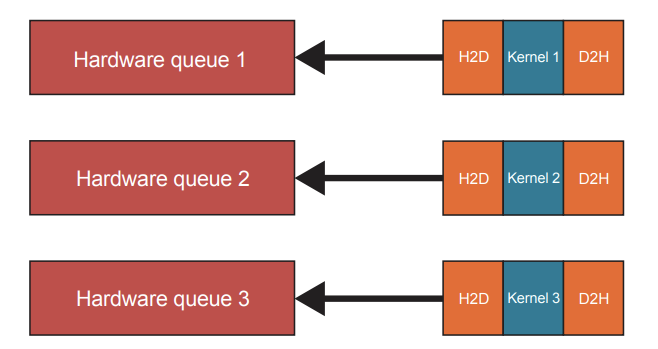
\includegraphics[width=0.8\linewidth]{FileAusiliari/Screenshots/Figure4-1.png}
    \caption{多個streams同時在GPU上進行記憶體複製與kernel啟動}
    \label{fig:lds}
\end{figure}

\subsection{同時執行的kernel}

來自不同streams的 kernels 可以同時執行,無論是在同個或不同的 GPU 上執行。如 Listing 4.9 所示,以下是一個host端程式碼的範例:首先,建立stream並完成host到device的資料傳輸。接著,分別在 Stream 1 和 Stream 2 上啟動兩個kernels。執行完成後,將輸出資料從device傳回host。這說明了使用 HIP stream來實現 kernel 層級並行是多麼容易的事情。本章提供的程式碼範例包括序列化 (\term{serial.cpp}) 和平行化 (\term{concurrent.cpp}) 兩種類型。我們還加入了測量這兩種實現效能的程式碼,鼓勵讀者透過stream實現較序列化執行 kernel 更高的效能。在 MI100 GPU 系統中,使用基於stream的並行 kernels 可實現最高達 2 倍的加速。此功能在 kernel 無法完全利用整個 GPU 資源時特別有幫助。

\begin{lstlisting}[language=C, caption={使用HIP stream的同時kernel -- host端}, label={9th:example}]
// 使用hipMalloc宣告所有的陣列
hipStream_t stream1, stream2;
hipStreamCreate(&stream1);
hipStreamCreate(&stream2);

HIP_ASSERT(hipMemcpy(&deviceA1,&A1, arraySize,hipMemcpyHostToDevice);
HIP_ASSERT(hipMemcpy(&deviceA2,&A2, arraySize,hipMemcpyHostToDevice);

square<<<gridSize, blockSize, 0, stream1>>>(deviceA1, deviceB1, n);
cube<<<gridSize, blockSize, 0, stream2>>>(deviceA2, deviceB2, n);

HIP_ASSERT(hipMemcpy(&B1 ,&deviceB1, arraySize, hipMemcpyDeviceToHost, stream1);
HIP_ASSERT(hipMemcpy(&B2, &deviceB2, arraySize, hipMemcpyDeviceToHost, stream2);
\end{lstlisting}

\begin{lstlisting}[language=C, caption={cube和square的kernel程式碼}, label={10th:example}]
__global__ void square(douvle *a, double *b, int n){
    // 取得我們的全域thread ID
    int id = blockIdx.x * blockDim.x + threadIdx.x;

    // 確保我們不會越界存取
    if(id < n)
        b[id] = a[id] * a[id];
}

__global__ void cube(double *a, double *b){
    // 取得我們的全域thread ID
    int id = blockIdx.x * blockDim.x + threadIdx.x;

    // 確保我們不會越界存取
    if(id < n)
        b[id] = a[id] * a[id] * a[id];
}
\end{lstlisting}

\subsection{重疊計算與溝通}
若我們可以利用streams的並行執行特性重疊計算與通信,我們便能縮短程式執行時間。藉由將計算任務和資料傳輸分配到不同的stream中,可以隱藏資料傳輸的延遲,因為跨stream的操作不會互相阻塞。這種技術對於大型問題和高資料傳輸需求特別有用,允許在 kernel 啟動之前進行資料的預傳輸。

一種常見的模式是將資料集劃分為多個子集並以流水線方式執行。stream透過允許每個stream處理資料的子集來促成這種模式。利用這種模式,可以加速 kernel 啟動並實現並行資料傳輸。透過優化計算和通信任務的管理,可以顯著提升效能。

讓我們重新審視 Listing 4.10 範例中的 cube kernel。首先,我們透過劃分資料集來減少問題規模。雖然在範例中選擇了四個stream,但我們鼓勵讀者嘗試其他分割設定。在範例中,我們將 1 億個輸入資料分割給四個stream,每個stream處理 2500 萬個資料。

一個常見的做法是利用 FOR 迴圈在多個stream中啟動 kernels,如 Listing 4.9 所示。首先,我們計算偏移量,用於識別與每個stream相關的資料子集。接下來,使用 \term{hipMemcpyAsync} 從host傳輸資料到device,利用上一步計算出的偏移量標記每個stream需要複製的資料區塊。這個 HIP 呼叫是非阻塞的,因此應用程式的下一行 (即kernel 啟動) 會立即到 GPU 排隊。需要注意的是,host完成 kernel 啟動指令的執行並不意味著 GPU 會立即執行 kernel。由於同一stream中的指令按順序執行,kernel 啟動會等待實際的記憶體複製完成。同樣地,下一個 \term{hipMemcpyAsync} 指令會由host指示到device排隊,但在該stream中的 kernel 完成執行之前,資料傳輸不會開始。在 FOR 迴圈的下一次迭代中,host會對剩餘的stream執行相同的步驟。透過stream,程式設計者可以巧妙地將問題分解,並分配到多個stream,以實現計算與通信之間的高效並行。舉例來說,假設 Stream 1 中的 kernel 已經完成了host到device的資料傳輸並開始執行。同時,Stream 2 所需的資料可以並行傳輸到 GPU。即使某一stream中的 kernel 已經飽和了 GPU 的所有著色器(shader)資源,這種方法仍然帶來好處。這裡的核心思想是,透過在stream間重疊計算與通信,而非等待所有資料傳輸完成後才開始計算,我們可以顯著地提升性能。

\begin{lstlisting}[language=C, caption={使用HIP streams呈現重疊計算與通信的host端程式碼}, label={11th:example}]
// 使用hipMallocHost宣告所有陣列

for(int i = 0; i < num_streams; i++){
    int offset = i * elements_per_stream;
    HIP_ASSERT(hipMemcpyAsync(&d_input1[offset], &h_input1[offset], bytes_per_stream, hipMemcpyHostToDevice, stream[i]);
    cube<<<gridSizePerStream,blockSize,0,streams[i]>>>(d_input1, d_output1,offset);
    HIP_ASSERT(hipMemcpyAsync(&h_output1[offset],&d_output1[offset], bytes_per_stream, hipMemcpyDeviceToHost,streams[i]));
}
\end{lstlisting}

在\term{compute\_comm\_overlap.cpp} 中的程式碼展示了一種情況 -- 數據被劃分到四個流中,並通過 FOR 迴圈啟動,如 Listing 4.11 所示。在 MI100 系統上,這種重疊計算與通信的stream的實現相比只使用預設stream的實現,達到了 4 倍的加速。因此,根據具體問題,程式設計者可以將大型問題分解為較小的stream,並重疊計算與通信,以獲得更高的性能。這種典型範例在許多機器學習框架中也很流行,例如 PyTorch \cite{paszke2019pytorch} 和 TensorFlow \cite{abadi2016tensorflow},因為它們常用流水線技術來實現神經網路的訓練與推理。

\section{HIP events (事件)}
我們可以通過在host程式碼中使用計時器或時鐘來檢查執行時間的測量過程。雖然這些方法可以提供基本的執行時間概念,但在測量 GPU 操作時,可能無法達到所需的準確性和可靠性。在本節中,我們將探討更高級的方法 -- HIP 事件,這是一種精確且可靠的測量 GPU 操作執行時間的方法。利用 HIP 事件,程式設計者可以有效識別性能瓶頸並優化程式碼以提高效率。

HIP 事件是監控 GPU 指令執行的強大工具。它們提供了精細的控制與執行時間的準確測量,使其成為性能分析中的重要元件。此外,我們將研究如何創建和使用 HIP 事件來準確測量向量加法操作,一個 GPU 程式設計中的基本任務的執行時間。HIP 事件在 HIP 程式設計模型中扮演至關重要的角色,為追踪 GPU 上執行的操作的狀態和進度提供了一種強大的機制。藉由\term{ hipEvent\_t} 類型,程式設計者可以獲得一組多功能的工具,用於有效監控任務的執行。\term{ hipEvent\_t} 類型是 HIP 程式設計中表示事件的基石,如 Listing 4.12 所示。通過使用該類型,程式設計者可以創建、記錄和同步事件,以精確控制 GPU 任務的執行流程。這種控制級別使得高效監控和分析 GPU 操作變得可能,從而幫助開發者優化程式碼並辨識性能瓶頸。

\begin{lstlisting}[language=C, caption={使用hipEvent\_t 型別}, label={12th:example}]
hipEvent_t
\end{lstlisting}

\subsection{創建HIP 事件}
在 GPU 程式設計中,HIP 事件作為一個強大的工具,用於在 GPU 上非同步記錄操作。通過使用 \term{hipEventCreate()} 函數,開發人員可以輕鬆地創建事件來捕捉執行時間線中的關鍵時刻,如 Listing 4.13 所示。HIP 事件的創建使程式設計者能夠深入瞭解 GPU 性能,成為 GPU 性能工程師。

\begin{lstlisting}[language=C, caption={使用hipEventCreate()創造事件}, label={13th:example}]
hipEventCreate(hipEvent_t *event)
\end{lstlisting}

\subsection{紀錄HIP 事件}
準確捕捉各種操作的開始和結束時間對於理解性能和優化程式碼至關重要。HIP 事件為實現此目標提供了一種高效且可靠的機制。通過使用 \term{hipEventRecord()} 函數,開發人員可以記錄包括數據傳輸和kernel執行等不同操作的時間邊界。在 \term{hipEventRecord()} 函數中,event 參數允許程式設計者指定需要記錄的 HIP 事件,而 stream 參數則指定記錄該事件的stream(如 Listing 4.14 所示)。通過策略性地放置這些函數調用,開發人員可以深入瞭解 GPU 操作的執行時間線。

\begin{lstlisting}[language=C, caption={使用hipEventRecord()紀錄HIP事件}, label={14th:example}]
hipEventRecord(hipEvent_t *event, hipStream_t stream))
\end{lstlisting}

\subsection{使用HIP 事件計算經過時間}
在軟體開發中,準確測量經過時間對於分析和優化性能非常重要。為了實現精確的時間測量,HIP 程式框架提供了一個強大的函數稱為 \term{hipEventElapsedTime()}。通過使用此函數,開發人員可以準確確認兩個事件之間的時間間隔。該函數接受三個參數:ms 是一個指向浮點變數的指標,用於接收計算出的經過時間;start 代表初始事件;stop 表示結束事件,如 Listing 4.15 所示。執行 \term{hipEventElapsedTime()} API 將返回一個以毫秒為單位的浮點值,允許開發人員捕捉指定事件之間的精確時間,並將其存儲在指定的變數中。

\begin{lstlisting}[language=C, caption={使用hipEventElapsedTime()計算經過時間}, label={15th:example}]
hipEventElapsedTime(float *ms, hipEvent_t start, hipEvent_t stop)
\end{lstlisting}

\subsection{結合HIP 事件與操作}
HIP API 中的另一個重要函數 \term{hipEventSynchronize()} 在stream同步中起著關鍵作用(如 Listing 4.16 所示)。當針對特定事件調用時,\term{hipEventSynchronize()} 會暫停host thread,直到相關事件以及相應stream中所有先前的操作完成執行為止。通過強制同步,此函數保證不同stream之間的事件按預期順序執行。\term{hipEventSynchronize()} 是協調操作的強大工具,可以消除競爭條件 (race condition) 並確保 GPU 任務執行的一致性。此函數為有效協調stream提供了手段,包括同步數據傳輸和kernel執行。

\begin{lstlisting}[language=C, caption={使用 hipEventSynchronize()
合併操作}, label={16th:example}]
hipEventSynchronize(hipEvent_t event)
\end{lstlisting}

\subsection{使用HIP 事件釋放記憶體}
高效的記憶體管理以確保高性能和資源利用,在程式設計是一個重要的方面。在 HIP 程式設計中,記憶體管理起著至關重要的作用。\term{hipEventDestroy()} 是管理 HIP 事件記憶體的一個重要函數,如 Listing 4.17 所示。此函數用於釋放與 HIP 事件相關聯的記憶體,從而釋放寶貴的資源並維持系統效率。在使用 \term{hipEventDestroy()} 時,開發者需要將事件操作器 (event handler) 作為參數傳遞,指定要釋放記憶體的事件。通過正確銷毀事件,程式設計者可以確保分配的記憶體被釋放,並供其他操作使用。

\begin{lstlisting}[language=C, caption={使用 hipEventDestroy()
釋放記憶體}, label={17th:example}]
hipEventDestroy(hipEvent_t event)
\end{lstlisting}

\subsection{使用特定標誌創建HIP 事件}
函數 \term{hipEventCreateWithFlags()} 用於搭配指定的標誌創建事件,並在device上為其分配記憶體,如 Listing 4.18 所示。此函數接受兩個參數:一個指向 \term{hipEvent\_t} 變數的指標,用於存儲創建的事件的把手 (handle);以及一個無符號整數,用於表示標誌。這些標誌可用於自定義事件的行為,例如指示事件應記錄於特定的stream中,或指定事件的完成類型。

\begin{lstlisting}[language=C, caption={使用 hipEventCreateWithFlags()
創建帶有標誌的事件}, label={18th:example}]
hipEventCreateWithFlags(hipEvent_t *event, unsigned flags)
\end{lstlisting}

\subsection{確保兩處理單元之間的一致性}
函數 \term{hipDeviceSynchronize()} 是 GPU 程式設計中一個重要的工具,可實現 CPU 與 GPU 之間的同步(見 Listing 4.19)。該函數是一個阻塞式呼叫,會暫停host(CPU)程式碼的執行,直到所有 GPU 的工作完成為止。通過使用 \term{hipDeviceSynchronize()},程式設計者可以確保在繼續後續的 CPU 操作之前,所有先前的 GPU 操作已經完成。這種同步機制對於需要依賴 GPU 所生成結果或數據的 CPU 程式碼特別有用。使用 \term{hipDeviceSynchronize()} 時,CPU 可以安全地等待 GPU 完成其工作量,從而保證數據在兩個處理單元之間的一致性和完整性。在執行 \term{hipDeviceSynchronize()} 期間,host thread會被暫停,使其能夠有效地追趕 GPU 的進度。該同步確保了 GPU 上不同stream中的所有操作都已完成,從而消除了潛在的競爭條件或數據不一致性問題。

\begin{lstlisting}[language=C, caption={使用 hipDeviceSynchronize()
確保兩個處理單元之間的一致性}, label={19th:example}]
hipDeviceSynchronize()
\end{lstlisting}

\subsection{使用HIP 事件的向量加法}
為了在實際案例中探索 hip 事件的使用,我們將重新審視向量加法範例。在第 2 章中的向量加法示例中,我們可以加入 hip 事件來測量 GPU 上的經過時間。首先,在 Listing 2.6 中的記憶體分配後,我們需要引入一個變數來存儲 GPU 經過的時間。接下來,使用 \term{hipEventCreate()} 函數創建兩個類型為 \term{hipEvent\_t} 的 HIP 事件,分別命名為 start 和 stop,如 Listing 4.20 所示。這些事件用於測量 GPU 計算期間的時間。通過創建這些事件,我們準備好測量 GPU 上的經過時間。然後,我們進行從 CPU 到 GPU 的記憶體複製,這與一般的向量加法示例相似。

\begin{lstlisting}[language=C, caption={GPU的記憶體配置與CPU到GPU的記憶體複製}, label={20th:example}]
// 此處宣告所有的GPU陣列
HIP_ASSERT(hipMalloc(&GPUArrayA, bytes));
HIP_ASSERT(hipMalloc(&GPUArrayB, bytes));
HIP_ASSERT(hipMalloc(&GPUArrayC, bytes));

float gpu_elapsed_time_ms;

hipEvent_t start, stop;
hipEventCreate(&start);
hipEventCreate(&stop);

// 將host向量複製到device
HIP_ASSERT(hipMemcpy(GPUArrayA, CPUArrayA, bytes, hipMemcpyHostToDevice));
HIP_ASSERT(hipMemcpy(GPUArrayB, CPUArrayB, bytes, hipMemcpyHostToDevice));
\end{lstlisting}

在記憶體複製完成、也在 Listing 2.4 中設置了kernel 啟動的block大小和grid大小後,我們可以開始使用 \term{hipEventRecord()} 函數來記錄 hip 事件。在這種情況下,我們將 start 變量作為參數傳遞,因為 \term{hipEventRecord()} 函數需要欲記錄的事件,如 Listing 4.21 所示。在使用 \term{hipEventRecord()} 啟動記錄後,我們啟動 kernel 以執行向量加法。一旦 kernel 執行完成,我們使用 stop 變量在 \term{hipEventRecord()} 函數中做停止記錄。為了確保同步和記錄事件的完成,我們使用 \term{hipEventSynchronize()} 函數與 stop 參數。同步完成後,我們通過將 GPU 記憶體複製回 CPU 記憶體來完成 kernel 執行。隨後,我們可以使用 \term{hipEventElapsedTime()} 函數來計算並印出 GPU 的經過時間,如 Listing 4.21 所示。最後,我們使用 free 和 hipFree 函數分別釋放host和device的記憶體。

\begin{lstlisting}[language=C, caption={組織 thread 與啟動 kernel}, label={21st:example}]
// 每個thread block中thread的數量
blockSize = 1024;
// grid中thread block的數量
gridSize = (int) ceil((float) b / blockSize);

hipEventRecord(start, 0);

// 執行kernel
vecAdd<<<gridSize,blockSize>>>(GPUArrayA,GPUArrayB,GPUArrayC,n);

hipEventRecord(stop, 0);
hipEventSynchronize(stop);

hipDeviceSynchronize();
HIP_ASSERT(hipMemcpy(CPUArrayC, GPUArrayC, bytes, hipMemcpyDeviceToHost));

hipEventElapsedTime(&gpu_elapsed_time_ms, start, stop);
printf("Time elapsed on vector addition on GPU: %f ms.\n\n", gpu_elapsed_time_ms);
\end{lstlisting}

通過結合 hip 事件,我們可以準確地測量向量加法範例中的 GPU 經過時間。通過記錄開始和停止事件、啟動 kernel 並同步這些事件,我們確保精確地測量 GPU 執行時間。利用 hipEventElapsedTime,我們可以計算並顯示這段時間。此外,適當的記憶體釋放確保了系統資源的高效利用。

\section{結語}
在本章中,我們介紹了 HIP 運行時 API 提供的更多進階功能。我們從討論 HIP 記憶體管理方法開始,因為適當的記憶體分配在 GPU 操作中尤其重要。在這個背景下,高效的記憶體傳輸和訪問是關鍵因素。接著,我們學習了 HIP stream的概念,一個能夠提升性能的強大工具。它們使得計算和通信可以同時進行,從而提高 GPU 和網路的利用率。在應用程式中根據 API 提供的方式使用 HIP stream ,既簡單又能顯著提升應用效率。最後,我們還討論了 HIP 事件,它在 GPU 同步和性能測量中扮演著至關重要的角色。它們提供了一種強而有力的方法來追蹤和監控在 GPU 上執行的操作。了解這些 HIP API 可以讓程式設計者以更加靈活且細緻的方式更好地控制 GPU。

% \bibliography{FileAusiliari/Bibliografia}